
\chapter{Wyniki działania algorytmu na popularnych zbiorach danych}

\section{Metodologia pomiarów}
	Żeby oszacować trafność klasyfikacji osiąganą przez skonstruowany system konieczne było podzielenie zbioru danych na zbiór uczący i \emph{walidujący}, a w przypadku algorytmu Kernel-GP również wydzielenie ze zbioru uczącego podzbioru \emph{testującego}, używanego do obliczania miary przystosowania (fitness) podczas przebiegu algorytmu genetycznego. Ponieważ sposób podziału zbioru danych ma wpływ na osiąganą trafność klasyfikacji, dokonywano 5 takich podziałów a następnie wyciągano średnią oraz odchylenie standardowe z wyników otrzymanych dla tych podziałów. Ta procedura dotyczyła zarówno testowania algorytmu \emph{Kernel-GP} jak i porównawczych testów klasyfikatora SVM z biblioteki \emph{LibSVM}. Dla obu algorytmów stosowano te same podziały danych, przy czym w przypadku klasyfikatora \emph{LibSVM} ze zbioru uczącego nie wydzielano zbioru testującego.
	
	Algorytm genetyczny jest w swej naturze stochastyczny, korzysta więc z funkcji generujących liczby pseudolosowe. Aby zapewnić powtarzalność wyników i umożliwić ich porównanie ziarno generatora liczb pseudolosowych ustawiono na stałą wartość.

	Aby ocenić skuteczność algorytmu genetycznego w poszukiwaniu optymalnych funkcji jądrowych oraz oszacować optymalną wielkość populacji, czas trwania algorytmu (liczbę ewaluowanych generacji) oraz najlepszą funkcję przystosowania przeprowadzono szereg eksperymentów obliczeniowych, w których uruchamiano algorytm dla coraz to większych wartości tych parametrów. Dla każdego przebiegu algorytmu obliczano i zapisywano kilka miar trafność klasyfikacji zbioru \emph{walidującego} (miary te zostały opisane w części \ref{sec:measures}).

	Analizując tak zebrane dane można przeanalizować na ile poszukiwanie funkcji jądrowej przez algorytm genetyczny było podobne do losowego przeszukiwania a na ile było ono zbieżne. W pierwszym przypadku na wyniki osiągane przez algorytm powinna mieć wpływ przede wszystkim wielkość populacji, w drugim również liczba generacji przez które poszukiwano rozwiązania. W szczególności ciekawym przypadkiem jest ten, gdy liczba generacji wynosi 1, czyli cały algorytm ogranicza się do wygenerowania populacji losowych osobników i wybrania jednego z nich - w tym przypadku algorytm genetyczny sprowadza się do losowego poszukiwania rozwiązania. Porównując różnicę w trafności osiąganej w trakcie jednej generacji i coraz większej ich liczby można ocenić czy proces ewolucyjny przebiega poprawnie. 
	
\section{Opis zbiorów danych}
	Do oceny pracy algorytmu użyto standardowych zbiorów danych służących do testowania systemów maszynowego uczenia się, dostępnych na stronie biblioteki \emph{LIBSVM} \cite{chang_libsvm:_2011}  oraz w repozytorium UCI  [\ref{url:uci}]. Zbiory zostały opisane w tabelce \ref{tab:datasets}. Użyte nazwy zbiorów są zgodne z tymi ze strony libsvm [\ref{url:libsvm}].

\begin{table}[ht]
	\caption{Zbiory danych użyte do testowania systemu.\label{tab:datasets}} 	
	\begin{tabular}{|p{2cm}|c|p{1.5cm}|p{1.5cm}|p{1.5cm}|p{1.5cm}|p{1.5cm}|}
		\hline 
		Nazwa zbioru & Liczba klas & \hspace{0pt} Liczba atrybutów & \hspace{0pt} Wielkość zbioru & \hspace{0pt} Wielkość zbioru uczącego & \hspace{0pt}Wielkość zbioru testującego & \hspace{0pt} Wielkość zbioru walidującego \\
		\hline 
		Iris & 3 & 4 & 150 & 68 & 33 & 49  \\ 
		\hline 
		Letter & 26 & 16 & 15000 & 9000 & 4400 & 6600\\ 
		\hline 
		DNA & 3 & 180 & 2000 & 1435 & 700 & 1051 \\ 
		\hline 
		Vowel & 11 & 10 & 528 & 447 & 217 & 326 \\ 
		\hline
		Breast cancer & 2 & 10 & 683 & 343 & 170 & 170 \\ 
		\hline
		Heart & 2 & 13 & 270 & 136 & 67 & 67 \\ 
		\hline
	\end{tabular} 	
\end{table}

\begin{table}[ht]
\caption{Zbiory danych użyte do testowania systemu.\label{tab:datasets2}} 	
	\begin{tabular}{|p{2.5cm}|p{2.5cm}|p{2.5cm}|p{1.5cm}|p{3cm}|}
	\hline 
	Nazwa zbioru & Liczba atrybutów ciągłych & Liczba atrybutów nominalnych & Liczba klas & Proporcje klas \\ 
	\hline 
	Breast Cancer & 10 & 0 & 2 & 239/444 \\ 
	\hline 
	Heart  & 7 & 6 & 2 & 150/120  \\ 
	\hline 
	DNA & 0 & 180 & 3 & 464/485/1051  \\ 
	\hline 
	Vowel & 10 & 0 & 11 & Każda klasa 48 razy \\ 
	\hline 
	\end{tabular} 
\end{table}


\FloatBarrier
\section{Fitness}
Aby ocenić dobór parametrów procesu ewolucyjnego zapisywano wartości fitness osiągane przez najlepszego osobnika w każdej generacji. Wartości te zostały przedstawione na wykresach przedstawiających wartość fitness najlepszego osobnika w funkcji czasu trwania algorytmu (ilości dotychczas wygenerowanych populacji), czyli tak zwanych \english{Fitness Graphs}. Na wykresash \ref{fig:fit-heart} - \ref{fig:fit-breast} widać jak zmienia się wartość funkcji fitness wraz z kolejnymi generacjami dla różnych miar jakości klasyfikacji użytych jako funkcja fitness (miary te zostały opisane w części \ref{sec:measures} a ich użycie w części \ref{sec:ewaluacja}).

	\begin{figure}
		\includegraphics[scale=0.90]{figures/results/fitness/fitness-heart}
		\caption{Najlepsza wartość funkcji przystosowania dla kolejnych generacji dla zbioru \emph{heart}.\label{fig:fit-heart}}
	\end{figure}
	
	\begin{figure}
		\includegraphics[scale=0.90]{figures/results/fitness/fitness-breast}
		\caption{Najlepsza wartość funkcji przystosowania dla kolejnych generacji dla zbioru \emph{breast}.\label{fig:fit-breast}}
	\end{figure}	

	
\FloatBarrier
\section{Wyniki klasyfikacji zbioru walidującego}
	Wyniki klasyfikacji zostały ocenione za pomocą miar opisanych w części \ref{sec:measures}. Dla każdej z tych miar przedstawiono jej wartości dla przebiegów algorytmu, w których jako funkcja fitness była wybrana właśnie ta miara. Dodatkowo na wykresach ukazano wartości danych miar uzyskane w wyniku klasyfikacji za pomocą trzech standardowych funkcji jądrowych (\emph{Wielomianowej}, \emph{Sigmoidalnej} i \emph{RBF}).
	
	Jak widać na rysunkach \ref{fig:acc-breast}-\ref{fig:probability-heart} sprawność algorytmu zależy zarówno od zbioru danych jak i od wybranej miary jakości.
	
	\begin{figure}
		\includegraphics[scale=0.90]{figures/results/accuracy/accuracy-breast}
		\caption{Tragność (\english{accuracy}) klasyfikacji dla zbioru \emph{breast} w funkcji czasu wykonania (ilości generacji).\label{fig:acc-breast}}
	\end{figure}
	
	\begin{figure}
		\includegraphics[scale=0.90]{figures/results/accuracy/accuracy-heart}
		\caption{Tragność (\english{accuracy}) klasyfikacji dla zbioru \emph{heart} w funkcji czasu wykonania (ilości generacji).\label{fig:acc-heart}}
	\end{figure}
	
	\begin{figure}
		\includegraphics[scale=0.90]{figures/results/f1/f1-breast}
		\caption{Wartość miary F1 dla wyników klasyfikacji zbioru \emph{breast} w funkcji czasu wykonania (ilości generacji).\label{fig:f1-breast}}
	\end{figure}
	
	\begin{figure}
		\includegraphics[scale=0.90]{figures/results/f1/f1-heart}
		\caption{Wartość miary F1 dla wyników klasyfikacji zbioru \emph{heart} w funkcji czasu wykonania (ilości generacji).\label{fig:f1-heart}}
	\end{figure}
	
	\begin{figure}
		\includegraphics[scale=0.90]{figures/results/mcc/mcc-breast}
		\caption{Wartość miary \emph{Mathews Correlation Coefficent} (\akronim{mcc}) dla wyników klasyfikacji zbioru \emph{breast} w funkcji czasu wykonania (ilości generacji).\label{fig:mcc-breast}}
	\end{figure}
	
	\begin{figure}
		\includegraphics[scale=0.90]{figures/results/mcc/mcc-heart}
		\caption{Wartość miary \emph{Mathews Correlation Coefficent} dla wyników klasyfikacji zbioru \emph{heart} w funkcji czasu wykonania (ilości generacji).\label{fig:mcc-heart}}
	\end{figure}
	
	\begin{figure}
		\includegraphics[scale=0.90]{figures/results/probability/probability-breast}
		\caption{Średnia wartość prawdopodobieństwa przypisywanego przez SVM właściwej dla klasyfikowanego przykłau klasie w funkcji czasu wykonania (ilości generacji). Zbiór \emph{breast}\label{fig:probability-breast}}
	\end{figure}
	
	\begin{figure}
		\includegraphics[scale=0.90]{figures/results/probability/probability-heart}
		\caption{Średnia wartość prawdopodobieństwa przypisywanego przez SVM właściwej dla klasyfikowanego przykłau klasie w funkcji czasu wykonania (ilości generacji). Zbiór \emph{heart}.\label{fig:probability-heart}}
	\end{figure}

%	\subsection{Porównanie z tradycyjnym algorytmem SVM}
%	Na wykresach \ref{fig:acc-iris-svm}-\ref{fig:acc-letter-svm} przedstawiono porównanie trafności klasyfikacji zbioru walidującego przez algorytm SVM z użyciem czterech podstawowych funkcji jądrowych (liniowej, wielomianowej, RBF i sigmoidalnej) i przez stworzony algorytm Kernel-GP.
%	W przypadku dwóch zbiorów: \emph{vowel} i \emph{letter} udało się uzyskać polepszenie trafności klasyfikacji względem standardowych funkcji jądrowych. Są to zbiory, dla których standardoy SVM osiąga słabe wyniki - ok. $ 70\% - 80\% $. 
%
%	W przypadku dwóch pozostałych zbiorów niezależnie od użytej funkcji jądrowej osiągana trafność klasyfikacji jest bardzo wysoka - ok. $ 95\% $ - sugeruje to, że zbiory te są dość łatwo separowalne z wyjątkiem $ 5\% $ przypadków.
	
%	\begin{figure}
%		\includegraphics[scale=0.90]{figures/results/accuracy/accuracy-iris-svm}
%		\caption{Porównanie dokładności klasyfikacji dla zbioru \emph{iris} przez algorytm SVM z różnymi funkcjami jądrowymi i algorytm Kernel-GP\label{fig:acc-iris-svm}}
%	\end{figure}
%	
%	\begin{figure}
%		\includegraphics[scale=0.90]{figures/results/accuracy/accuracy-dna-svm}
%		\caption{Porównanie dokładności klasyfikacji dla zbioru \emph{dna} przez algorytm SVM z różnymi funkcjami jądrowymi i algorytm Kernel-GP.\label{fig:acc-dna-svm}}
%	\end{figure}	
%	
%	\begin{figure}
%		\includegraphics[scale=0.90]{figures/results/accuracy/accuracy-vowel-svm}
%		\caption{Porównanie dokładności klasyfikacji dla zbioru \emph{vowel} przez algorytm SVM z różnymi funkcjami jądrowymi i algorytm Kernel-GP\label{fig:acc-vowel-svm}}
%	\end{figure}
%	
%	\begin{figure}
%		\includegraphics[scale=0.90]{figures/results/accuracy/accuracy-letter-svm}
%		\caption{Porównanie dokładności klasyfikacji dla zbioru \emph{letter} przez algorytm SVM z różnymi funkcjami jądrowymi i algorytm Kernel-GP\label{fig:acc-letter-svm}}
%	\end{figure}		

\FloatBarrier
	\subsection{Monotoniczność funkcji trafności}	
	Miejscami funkcja trafności nie jest monotoniczna, a ściślej niemalejąca, względem liczby generacji oraz wielkości populacji (co widać np. na wykresach \ref{fig:acc-iris-detailed} i \ref{fig:acc-vowel-detailed}). Wydawałoby się, że tak być nie powinno (algorytm genetyczny zwraca najlepszego osobnika z całego swojego przebiegu, więc wszystkie osobniki, które pojawiły się podczas przebiegu z 5 generacjami pojawią się podczas przebiegu z 7 generacjami, więc trafność dla przebiegu z 7 generacjami powinna być co najmniej tak dobra jak dla przebiegu z 5 generacjami). Jednak może się tak zdarzyć ze względu na to, że trafność pokazana na wykresach to trafność klasyfikacji zbioru walidującego, natomiast trafność użyta przez algorytm genetyczny jako miara dostosowania (\english{fitness}) to trafność klasyfikacji zbioru testującego. Widać to na wykresie \ref{fig:fit-iris-detailed}, który przedstawia wartość przystosowania dla tych samych danych, dla których na wykresie \ref{fig:acc-iris-detailed} jest pokazana trafność klasyfikacji na zbiorze walidującym - tutaj funkcja wykazuje mniej braku monotoniczności. 

%	\begin{figure}
%		\includegraphics[scale=0.90]{figures/results/accuracy/accuracy-iris}
%		\caption{Dokładność klasyfikacji dla zbioru \emph{iris} w funkcji rozmiaru populacji dla róznych ilości generacji.\label{fig:acc-iris}}
%	\end{figure}
%	
	\begin{figure}
		\includegraphics[scale=0.90]{figures/results/accuracy/accuracy-iris-detailed}
		\caption{Dokładność klasyfikacji dla zbioru \emph{iris} w funkcji rozmiaru populacji dla róznych ilości generacji, dla małych populacji.	\label{fig:acc-iris-detailed}}
	\end{figure}	
	
	
	\begin{figure}
		\includegraphics[scale=0.90]{figures/results/fitness/fitness-iris-detailed}
		\caption{Najlepsza wartość funkcji przystosowania (\english{fitness})  \emph{iris} w funkcji rozmiaru populacji dla róznych ilości generacji, dla małych populacji.	\label{fig:fit-iris-detailed}}
	\end{figure}	
	
%	
%	\begin{figure}
%		\includegraphics[scale=0.90]{figures/results/accuracy/accuracy-dna}
%		\caption{Dokładność klasyfikacji dla zbioru \emph{DNA} w funkcji rozmiaru populacji dla róznych ilości generacji.\label{fig:acc-dna}}
%	\end{figure}
%	
%	\begin{figure}
%		\includegraphics[scale=0.90]{figures/results/accuracy/accuracy-dna-detailed}
%		\caption{Dokładność klasyfikacji dla zbioru \emph{DNA} w funkcji rozmiaru populacji dla róznych ilości generacji, dla małych populacji.\label{fig:acc-dna-detailed}}
%	\end{figure}	
%	
%
%	\begin{figure}
%		\includegraphics[scale=0.90]{figures/results/accuracy/accuracy-vowel}
%		\caption{Dokładność klasyfikacji dla zbioru \emph{vowel} w funkcji rozmiaru populacji dla róznych ilości generacji.\label{fig:acc-vowel}}
%	\end{figure}
		%	
%	
%		\begin{figure}
%		\includegraphics[scale=0.90]{figures/results/accuracy/accuracy-letter}
%		\caption{Dokładność klasyfikacji dla zbioru \emph{letter} w funkcji rozmiaru populacji dla róznych ilości generacji.\label{fig:acc-letter}}
%	\end{figure}
%	
%		
%	\begin{figure}
%		\includegraphics[scale=0.90]{figures/results/accuracy/accuracy-letter-detailed}
%		\caption{Dokładność klasyfikacji dla zbioru \emph{letter} w funkcji rozmiaru populacji dla róznych ilości generacji, dla małych populacji.\label{fig:acc-letter-detailed}}
%	\end{figure}
%	

	\FloatBarrier
	Zatem przynajmniej część braku monotoniczności funkcji trafności na zbiorze walidującym wynika z przeuczenia algorytmu - znaleziona przez algorytm genetyczny funkcja jądrowa lepiej sprawdza się przy klasyfikacji zbioru testującego niż walidującego. Nie jest to jednak jedyna przyczyna braku monotoniczności - widać to na wykresie \ref{fig:fit-vowel-detailed} przedstawiającym wartość funkcji przystosowania dla zbioru \emph{vowel} - jej przebieg jest bardzo podobny do przebiegu ukazanej na rys. \ref{fig:acc-vowel-detailed} funkcji trafności klasyfikacji zbioru walidującego na tym samym zbiorze. Co więc jest przyczyną braku monotoniczności? Warto zauważyć, że funkcja jest niemalejąca ze względu na ilość generacji oraz że dla jednej generacji funkcja jest monotoniczna. Sugeruje to, że "winnym" może być selekcja - w praktyce nie zachodzi ono w przypadku gdy algorytm genetyczny działa przez jedną generację.

	\begin{figure}
		\includegraphics[scale=0.90]{figures/results/accuracy/accuracy-vowel-detailed}
		\caption{Dokładność klasyfikacji dla zbioru \emph{vowel} w funkcji rozmiaru populacji dla róznych ilości generacji, dla małych populacji.\label{fig:acc-vowel-detailed}}
	\end{figure}
		
	\begin{figure}
		\includegraphics[scale=0.90]{figures/results/fitness/fitness-vowel-detailed}
		\caption{Dokładność klasyfikacji dla zbioru \emph{vowel} w funkcji rozmiaru populacji dla róznych ilości generacji, dla małych populacji.\label{fig:fit-vowel-detailed}}
	\end{figure}

    	
	\FloatBarrier
	 Gdy przyjrzeć się dokładnie przebiegowi ewolucji widać, że rzeczywiści tak jest. Dodatkowy osobnik (rys. \ref{fig:func1}), który odróżnia w generacji pierwszej populacje o wielkości 3 i 4 jest przodkiem innego osobnika (rys. \ref{fig:func2}), który w trzeciej generacji osiąga fitness większy niż osobnik (rys. \ref{fig:func3}), który w przypadku populacji wielkości 3 był przodkiem osobnika (rys. \ref{fig:func4}), który to okazał się najlepszym podczas przebiegu całego algorytmu. W rezultacie tego "geny" potencjalnego zwycięzcy nie przetrwały w przebiegu algorytmu z populacją liczącą 4 osobników. Jak widać osobnik najlepszy we wszystkich generacjach nie musi być wcale potomkiem osobników najlepszych w poszczególnych generacjach - czasem połączenie dwóch osobników przeciętnych może dać osobnika bardzo dobrego. 	
	 
	     \begin{figure}
		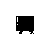
\includegraphics[scale=0.50]{figures/functions/func1}
		\caption{Funkcja z pierwszej generacji, która w przebiego z wielkością populacji 4 osiągnęła fitness $0.4242424$. Przodek funkcji z rys.\ref{fig:func2} \label{fig:func1}}
	\end{figure}
	
	\begin{figure}
		\includegraphics[scale=0.60]{figures/functions/func2}
		\caption{Funkcja z trzeciej generacji, która w przebiego z wielkością populacji 4 osiągnęła fitness $0.78030306$. Potomek funkcji z rys.\ref{fig:func1}, przodek zwycięskiej funkcji (rys.\ref{fig:func5}) z przebiegu z populacją o wielkości 4.\label{fig:func2}}
	\end{figure}
          
   	\begin{figure}
		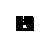
\includegraphics[scale=0.60]{figures/functions/func5}
		\caption{Funkcja z ostatniej generacji w przebiegu z wielkością populacji 4 osiągnęła fitness $0.8333333$. Przodek zwycięskiej funkcji z rys.\ref{fig:func4} \label{fig:func5}}
	\end{figure}          


   	\begin{figure}
		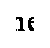
\includegraphics[scale=0.60]{figures/functions/func3}
		\caption{Funkcja z trzeciej generacji, która w przebiegu z wielkością populacji 3 i 4 osiągnęła fitness $0.6515151$. Przodek zwycięskiej funkcji z rys.\ref{fig:func4}\label{fig:func3}}
	\end{figure}                 

    	\begin{figure}
		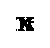
\includegraphics[scale=0.60]{figures/functions/func4}
		\caption{Zwycięska funkcja w przebiegu z populacją wielkości 3, potomek funkcji z rys.\ref{fig:func3}. Osiągnęła fitness $0.9015151$. \label{fig:func4}}
	\end{figure} 


		


\section{Czas wykonania}

\section{Użycie pamięci}

\section{Posdumowanie wyników}

\clearpage
